
%{{{ Preamble

%\documentclass[draft]{beamer} %% normal document
\documentclass[]{beamer} %% normal document
\usepackage{fontspec, unicode-math, caption, float, filecontents, verbatim}
\usepackage[english]{babel}

%{{{ Beamer Stuff

\usetheme{Frankfurt}
\useoutertheme{split}
\useinnertheme{rectangles}
%%\definecolor{bettergreen}{rgb}{.1,.7,.1}
%%\usecolortheme[named=bettergreen]{beaver}

\definecolor{bettergreen}{rgb}{0.1,0.7,0.1}

%\usetheme{Dresden}
%\usecolortheme[named=bettergreen]{structure}
\usecolortheme[named=bettergreen]{structure}

\setbeamercolor{section in head/foot}{fg=green, bg=black}
\setbeamercolor{section shaded}{fg= grey}


%\setbeamertemplate{caption}[numbered]
%\captionsetup{labelformat=simple,font=scriptsize,labelfont=scriptsize}
\beamertemplatenavigationsymbolsempty

% puts Frame numbers in Dresden template
\newcommand*\oldmacro{}%
\let\oldmacro\insertshorttitle%
\renewcommand*\insertshorttitle{%
	\oldmacro\hfill%
\insertframenumber\,/\,\inserttotalframenumber}

%\logo{\pgfimage[width=2cm,height=2cm]{material/schlangenlogo}}
\newcommand{\nologo}{\setbeamertemplate{logo}{}} % command to set the logo to nothing


\AtBeginSection[]
{%
	\begin{frame}<beamer>
		\frametitle{Table of Contents}
		\tableofcontents[currentsection]
		%\tableofcontents
	\end{frame}
}




%}}}

\newcommand{\as}[1]{{\fontspec{ProFontWindows} \textcolor{white}{#1} } }
\newcommand{\source}[1]{{\caption{\tiny {\fontspec{ProFontWindows} {Source: #1} } } } }
\newcommand{\sources}[1]{{\caption{\tiny {\fontspec{ProFontWindows} {Sources: #1} } } } }
\newcommand{\greenbullet}{\textcolor{bettergreen}\textbullet}
%\newcommand{\greencirc}{\textcolor{bettergreen} $ \circ $}
\newcommand{\greencirc}{$ \circ $ }

\usepackage{multicol}

\usepackage{tikz}
\usetikzlibrary{arrows, decorations.markings}
\usetikzlibrary{positioning,shapes,shadows,calc,positioning}
\usetikzlibrary{decorations.pathreplacing,angles,quotes}
\usetikzlibrary{decorations.pathmorphing}
%\usetikzlibrary{fit}


% This part taken from http://www.texample.net/tikz/examples/double-arrows/
% Double Arrows a la Chef
% Author: Dominik Haumann

% for double arrows a la chef
% adapt line thickness and line width, if needed
%\tikzstyle{vecArrow} = [thick, decoration={markings,mark=at position
%   1 with {\arrow[semithick]{open triangle 60}}},
%   double distance=1.4pt, shorten >= 5.5pt,
%   preaction = {decorate},
%   postaction = {draw,line width=1.4pt, white,shorten >= 4.5pt}]
%\tikzstyle{innerWhite} = [semithick, white,line width=1.4pt, shorten >= 4.5pt]


%\tikzstyle{mynode} = [rectangle,rounded corners,draw=black,top color=white, bottom color=white!50,very thick, inner sep=1em, minimum size=3em, text centered]
%\tikzstyle{invnode} = [inner sep=0,minimum size=0]
%
%\tikzstyle{abstract}=[rectangle, draw=black, rounded corners, fill=blue!40, drop shadow, text centered, anchor=north, text=white, text width=3cm]
%\tikzstyle{comment}=[rectangle, draw=black, rounded corners, fill=green, drop shadow, text centered, anchor=north, text=white, text width=3cm]
%\tikzstyle{myarrow}=[->, >=open triangle 90, thick]
%\tikzstyle{line}=[-, thick]


\tikzset{font={\fontsize{8pt}{7}\selectfont}}
\tikzset{every picture/.append style={scale=0.1}}


\usepackage{etex} %% Cool Stuff, see http://tex.stackexchange.com/a/36721/69074 : \foreach \i in {0,...,\number\numexpr\memBlocks-1\relax}
\newcommand{\CC}{C\nolinebreak\hspace{-.05em}\raisebox{.4ex}{\tiny\bf +}\nolinebreak\hspace{-.03em}\raisebox{.4ex}{\tiny\bf +}}




%{{{ Extract Coordinates

% http://tex.stackexchange.com/a/179946/69074
\makeatletter
\def\extractcoord#1#2#3{%
  \path let \p1=(#3) in \pgfextra{%
    \pgfmathsetmacro#1{\x{1}/\pgf@xx}%
    \pgfmathsetmacro#2{\y{1}/\pgf@yy}%
    \xdef#1{#1} \xdef#2{#2}%
  };%
}%
\makeatother

\newcommand*{\LabelCoord}[4]{\fill [#1] ($(#2,#3)$) circle (2pt) node [right] {#4}}%
%}}}


% For image1
\newif\iffourway

% For image3
\newif\ifshowreq
\newif\ifshowwb





%{{{ inputfile

% source: http://tex.stackexchange.com/questions/40738/how-to-properly-make-a-latex-project
\newcommand\inputfile[1]{%
    \InputIfFileExists{#1}{}{\typeout{No file #1.}}%
}


%\newcommand*{\COMPILEIMAGES}{}%


% Whether to compile the image-lets or include the pre-compiled ones
\newcommand*{\COMPILEIMAGES}{}%

\newcommand\inputimage[1]}}

%{{{ Avebritations

\usepackage{xspace}
\newcommand{\twi}{I\textsuperscript{2}C\xspace}
\newcommand{\mosi}{\texttt{MOSI}\xspace}
\newcommand{\miso}{\texttt{MISO}\xspace}
\newcommand{\clock}{\texttt{CLOCK}\xspace}
\renewcommand{\ss}{\texttt{\textoverline{SS}}\xspace}

\newcommand{\sda}{\texttt{SDA}\xspace}
\newcommand{\scl}{\texttt{SCL}\xspace}
\newcommand{\startcondition}{\texttt{START} condition\xspace}
\newcommand{\stopcondition}{\texttt{STOP} condition\xspace}
\newcommand{\clockstretching}{\texttt{CLOCK STRETCHING}\xspace}
\newcommand{\ack}{\texttt{ACK}\xspace}
\newcommand{\nak}{\texttt{NACK}\xspace}
%}}}

%{{{ MINTED

\usepackage{minted}
\definecolor{bg}{rgb}{0.95,0.95,0.95}
%\newminted[C++]{cpp}{numbersep=5pt, bgcolor=bg, gobble=0, linenos, tabsize=4}
%\newminted[C++]{cpp}{tabsize=4, obeytabs}
%}}} Minted

%{{{ Hyperref

\usepackage{hyperref}
\definecolor{darkblue}{rgb}{0,0,.5}
%linkcolor will also affect the text in the navigation bar on the top of each slide
%\hypersetup{pdftex=true, colorlinks=true, breaklinks=true, linkcolor=darkblue, menucolor=darkblue, pagecolor=darkblue, urlcolor=darkblue}
\hypersetup{pdfpagemode=FullScreen}
%}}}

%{{{ Animate

%%\usepackage[controls, autoplay]{animate}
%\usepackage[autoplay]{animate}
%%\animategraphics[<options>]{<frameand the environment rate>}{<file basename>}{<first>}{<last>}
%}}}

%{{{ Changemargin

\newenvironment{changemargin}[2]
{
	\begin{list}{}
		{
			\setlength{\topsep}{0pt}
			\setlength{\leftmargin}{#1}
			\setlength{\rightmargin}{#2}
			\setlength{\listparindent}{\parindent}
		\setlength{\itemindent}{\parindent}
			\setlength{\parsep}{\parskip}
		}
	\item[]
	}
	{
	\end{list}
}
%}}}

%{{{ Graphics Loading

\usepackage{graphicx}
\graphicspath{{../material/presentation/}{../material/background/}}
\usepackage{caption}
\captionsetup[figure]{labelformat=empty, font=scriptsize, justification=raggedleft, singlelinecheck=false}% redefines the caption setup of the figures environment in the beamer class.
%}}}

%{{{ Tkz drawing package

%{{{ Block diagram

\usepackage{tikz}
\usetikzlibrary{arrows, decorations.markings, positioning}

% for double arrows a la chef
% adapt line thickness and line width, if needed
\tikzstyle{vecArrow} = [thick, decoration={markings,mark=at position
	1 with {\arrow[semithick]{open triangle 60} } },
	double distance=1.4pt, shorten >= 5.5pt,
	preaction = {decorate},
postaction = {draw,line width=1.4pt, white,shorten >= 4.5pt}]
\tikzstyle{innerWhite} = [semithick, white,line width=1.4pt, shorten >= 4.5pt]
%}}}

%{{{ Tkz timing package

\usepackage{tikz-timing}
%\usetikztiminglibrary{nicetabs} % a bit strange with \Huge; use belowrulesep to adjust
%}}}

%}}}

%{{{ Fullpage

\newenvironment{fullpage}[0]{%
	\begin{list}{}{%
		\setlength{\leftmargin}{-7mm}%
		\setlength{\rightmargin}{-7mm}%
		\vspace*{-10pt}
		}%
\item[]}{\end{list}}
%}}}


%{{{ Title

\title[]{RISC V - Architecture and Interfaces}
\subtitle[]{The RocketChip}
%\subject{}
\keywords{RISCV, RocketChip}
\date{\today}
%}}}

%{{{ Author

\author{Moritz~Nöltner-Augustin}
\institute[ZITI]}}

%}}}




%{{{
\begin{document}

%{{{ Titlepage

\begin{frame}[plain]
	\titlepage
	%\note{}
\end{frame}
%}}}

%{{{ Table of Contents

\begin{frame}<beamer>
	\frametitle{Table of Contents}
	\tableofcontents
\end{frame}
%}}}




%{{{
\section{Introduction}

%{{{
\begin{frame}{What is RISCV?}
	\begin{figure}
		\centering{
\includegraphics[width=0.80\pagewidth,height=0.80\pageheight,keepaspectratio]{riscv-logo}}
		\vspace*{-0.1cm}
		\source{\url{https://riscv.org}}
	\end{figure}
	\begin{columns}
		\column{0.5\textwidth}
		\begin{itemize}
			\item Open-source Instruction Set Architecture (ISA)
			\item One ISA to cover all computer devices
			\item 3 ISAs (32-128 bits)
			\item Meant for implementation
		\end{itemize}
		\column{0.5\textwidth}
		\begin{itemize}
			\item Modular
			\item Extensible
			\item Actively developed
			\item A good investment?
		\end{itemize}
	\end{columns}
\end{frame}
%}}}

%{{{
\begin{frame}{Why should I care?}
	\begin{columns}
		\column{0.7\textwidth}
		lowRISC aims to create the processor pendant of linux
		\column{0.3\textwidth}
	\begin{figure}
		\centering{
\includegraphics[width=0.15\pagewidth,height=0.80\pageheight,keepaspectratio]{lowrisc}}
	\end{figure}
	\end{columns}
	\begin{columns}
		\column{0.3\textwidth}
	\begin{figure}
		\centering{
\includegraphics[width=0.20\pagewidth,height=0.80\pageheight,keepaspectratio]{sifive}}
	\end{figure}
		\column{0.7\textwidth}
		SiFive and Open-V create custom silicon
	\end{columns}
	\begin{columns}
		\column{0.7\textwidth}
		ETH Zurich and Università di Bologna create a state of the art microcontroller
		\column{0.3\textwidth}
	\begin{figure}
		\centering{
\includegraphics[width=0.20\pagewidth,height=0.80\pageheight,keepaspectratio]{pulp}}
	\end{figure}
	\end{columns}
	\begin{columns}
		\column{0.33\textwidth}
		\begin{itemize}
			\item Nvidia replaces Falcon processor
		\end{itemize}
		\column{0.33\textwidth}
		\begin{itemize}
			\item IIT Madras creates a processor
		\end{itemize}
		\column{0.33\textwidth}
		\begin{itemize}
			\item UC Berkeley uses it for reasearch
		\end{itemize}
	\end{columns}
	\begin{figure}
		\sources{\cite{riscv_users}}
	\end{figure}
\end{frame}
%}}}


%}}} End: section{Introduction}


%{{{
\section{Structure}

%{{{
\begin{frame}{What is RocketChip?}
	\begin{figure}
		\centering{
		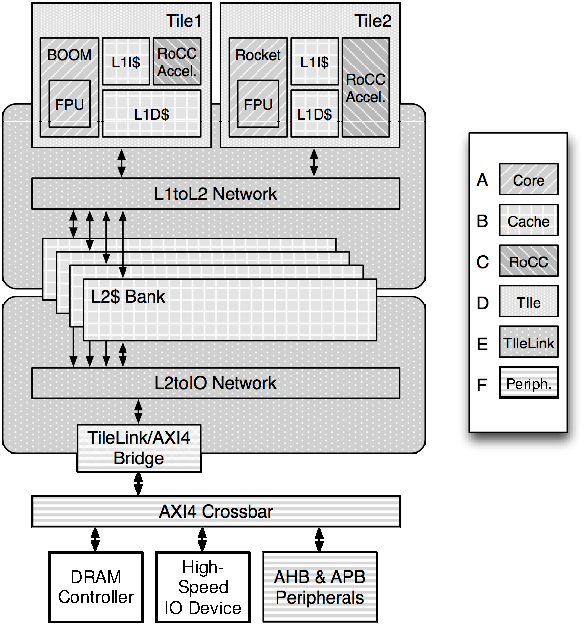
\includegraphics[width=0.90\pagewidth,height=0.80\pageheight,keepaspectratio]{EECS-2016-17_fig1}
		}
		\vspace*{-1cm}
		\source{\cite{rc_paper}}
	\end{figure}
\end{frame}
%}}}

%{{{
\begin{frame}[fragile]{How can I "use" RocketChip?}
	%\begin{minipage}[c][.4\textheight][c]{\linewidth}
		\begin{figure}
			\begin{minted}[fontsize=\small, gobble=4]{bash}
				git clone https://github.com/ucb-bar/rocket-chip.git
				cd rocket-chip
				#git checkout boom
				git submodule update --init --recursive
				# Now the repo is about 3GB
				cd riscv-tools
				export RISCV=/path/to/toolchain/install
				export PATH="${PATH}:$RISCV/bin"
				./build.sh # Takes about 45 min
				# The toolchain is another 800MB
				cd ../emulator
				make run CONFIG=BOOMConfig
				make run CONFIG=ExampleSmallConfig
				cd ../vsim
				make -jN CONFIG=ExampleSmallConfig # about 20 min
			\end{minted}
			\source{Collected from \cite{rc_github} and \cite{boom_github}}
		\end{figure}
	%\end{minipage}
\end{frame}
%}}}

%{{{
\begin{frame}[fragile]{What can be configured?}
	\begin{fullpage}
		A selection from \$(ROCKET-CHIP)/src/main/scala/coreplex/Configs.scala:
		\vspace{3mm}
	\begin{columns}
		\column{0.33\textwidth}
			Tile (RC || Boom):
		\column{0.33\textwidth}
			Caches:
		\column{0.33\textwidth}
			Uncore:
	\end{columns}
	\begin{columns}
		\column{0.33\textwidth}
			\begin{itemize}
				\item Instruction width
				\item IFetch width
				\item Use debug
				\item \#Breakpoints
				\item \#Perf. Counters
				\item FPU key
				\item Mult. div. key
				\item Use atomics
			\end{itemize}
		\column{0.33\textwidth}
			\begin{itemize}
				\item \#Sets
				\item \#Ways
				\item \#TLB-Entries
				\item \#row bits
				\item \#id bits
				\item split metadata
				\item ECC code
				\item Replacement policy
			\end{itemize}
		\column{0.33\textwidth}
			\begin{itemize}
				\item TileLink config
				\item L1toL2 config
				\item Broadcast config
				\item Banked L2 config
				\item Bootrom
				\item \#Tiles
				\item \$block \#bytes
				\item Build Core?
			\end{itemize}
	\end{columns}
	\end{fullpage}
\end{frame}
%}}}

%{{{
\begin{frame}[fragile]{How to configure RocketChip? /1}
	\begin{fullpage}
		\$(RC)/src/main/scala/coreplex/Configs.scala:
		\begin{minted}[fontsize=\small, gobble=3, tabsize=2]{java}
			case CacheBlockBytes => 64
			case CacheName("L1D") => CacheConfig(
				nSets         = 64,
				nWays         = 4,
				rowBits       = site(L1toL2Config).beatBytes*8,
				nTLBEntries   = 8,
				cacheIdBits   = 0,
				splitMetadata = false)
			...
			class WithL1ICacheSets(sets:Int) extends Config((site,here,up)=>{
			 case CacheName("L1I")=>up(CacheName("L1I"), site).copy(nSets=sets)
			}) // Likewise for nWays
			class WithCacheBlockBytes(linesize:Int)
											extends Config((site,here,up)=>{
			 case CacheBlockBytes => linesize
			})
		\end{minted}
	\end{fullpage}
\end{frame}
%}}}

%{{{
\begin{frame}[fragile]{How to configure RocketChip? /2}
	\begin{fullpage}
	\$(ROCKET-CHIP)/src/main/scala/rocketchip
		\begin{minted}[fontsize=\small, gobble=3, tabsize=2]{java}
			class DualCoreConfig2way extends Config(
				new WithNCores(2) ++ new WithL1ICacheWays(2)
				++ new WithL1ICacheSets(32) ++ new WithCacheBlockBytes(64)
				++ new WithL2Cache ++ new BaseConfig)

			class DualCoreConfig4way extends Config(
				new WithNCores(2) ++ new WithL1ICacheWays(4)
				++ new WithL1ICacheSets(64) ++ new WithCacheBlockBytes(32)
				++ new WithL2Cache ++ new BaseConfig)
		\end{minted}
		\pause
		\begin{minted}[fontsize=\small, gobble=3]{bash}
			...
			cd rocket-chip/vsim
			make -j5 CONFIG=DualCoreConfig2way
			...
			make -j5 CONFIG=DualCoreConfig4way
		\end{minted}
	\end{fullpage}
\end{frame}
%}}}

%{{{
\begin{frame}{Cache Example, 2-Way}
	\begin{fullpage}
		\fourwayfalse
		%\centering
		\inputimage{image1}
	\end{fullpage}
\end{frame}
%}}}

%{{{
\begin{frame}{Cache Example, 4-Way}
	\begin{fullpage}
		\fourwaytrue
		%\centering
		\inputimage{image1}
	\end{fullpage}
\end{frame}
%}}}

%{{{
\begin{frame}[fragile,t]{Results: Module ICache\_icache (2 ways, 32 sets, 64 bytes)}
	\begin{fullpage}
	\begin{columns}
		\column{0.5\textwidth}
		\begin{minipage}[t][\textheight][l]{\linewidth}
			\begin{minted}[fontsize=\small, gobble=4, tabsize=2]{verilog}
				module tag_array( // x1
					input  [4:0] RW0_addr,
					input   RW0_en,
					input   RW0_clk,
					input   RW0_wmode,
					input  [20:0] RW0_wdata_0,
					input  [20:0] RW0_wdata_1,
					output [20:0] RW0_rdata_0,
					output [20:0] RW0_rdata_1,
					input   RW0_wmask_0,
					input   RW0_wmask_1
				);
				reg [41:0] ram [31:0];
			\end{minted}
		\end{minipage}
		\column{0.5\textwidth}
		\begin{minipage}[t][\textheight][l]{\linewidth}
			\begin{minted}[fontsize=\small, gobble=4, tabsize=2]{verilog}
				module _T_772( // x2
					input  [7:0] RW0_addr,
					input   RW0_en,
					input   RW0_clk,
					input   RW0_wmode,
					input  [63:0] RW0_wdata,
					output [63:0] RW0_rdata
				);
				reg [63:0] ram [255:0];
			\end{minted}
		\end{minipage}
	\end{columns}
	\end{fullpage}
\end{frame}
%}}}

%{{{
\begin{frame}[fragile,t]{Results: Module ICache\_icache (4 ways, 64 sets, 32 bytes)}
	\begin{fullpage}
	\begin{columns}
		\column{0.5\textwidth}
		\begin{minipage}[t][\textheight][l]{\linewidth}
			\begin{minted}[fontsize=\small, gobble=4, tabsize=2]{verilog}
				module tag_array( // x1
					input  [5:0] RW0_addr,
					input   RW0_en,
					input   RW0_clk,
					input   RW0_wmode,
					input  [20:0] RW0_wdata_0,
					input  [20:0] RW0_wdata_1,
					input  [20:0] RW0_wdata_2,
					input  [20:0] RW0_wdata_3,
					output [20:0] RW0_rdata_0,
					output [20:0] RW0_rdata_1,
					output [20:0] RW0_rdata_2,
					output [20:0] RW0_rdata_3,
					input   RW0_wmask_0,
					input   RW0_wmask_1,
					input   RW0_wmask_2,
					input   RW0_wmask_3
				);
				reg [83:0] ram [63:0];
			\end{minted}
		\end{minipage}
		\column{0.5\textwidth}
		\begin{minipage}[t][\textheight][l]{\linewidth}
			\begin{minted}[fontsize=\small, gobble=4, tabsize=2]{verilog}
				module _T_850( // x4
					input  [7:0] RW0_addr,
					input   RW0_en,
					input   RW0_clk,
					input   RW0_wmode,
					input  [63:0] RW0_wdata,
					output [63:0] RW0_rdata
				);
				reg [63:0] ram [255:0];
			\end{minted}
		\end{minipage}
	\end{columns}
	\end{fullpage}
\end{frame}
%}}}


%}}} End: section{Structure and Interfaces}


%{{{
\section{Interfaces}
%Note: AXI4... does not mean axi for ... but is the protocol version, AXI4.

%{{{
\begin{frame}{RocketChip Interfaces}
	\begin{fullpage}
		\small
		\begin{columns}
			\column{0.45\textwidth}
			\inputimage{image2}
			\column{0.55\textwidth}
			\pause
			\begin{itemize}
				\item 451 signals per TileLink
				\item TileLink: Data + Opcode
				\item 282 signals per AXI interface
				\item io\_l2\_axi4\_0 optional
			\end{itemize}
			\vspace{5mm}
			\begin{tabular}{l|l}
				Signal Bundle & Prefix\\
				\hline
				Write Address Channel & \ldots\_aw\_\ldots \\
				Write Data Channel & \ldots\_w\_\ldots \\
				Write Response & \ldots\_b\_\ldots \\
				Read Address Channel & \ldots\_ar\_\ldots \\
				Read Data Channel & \ldots\_r\_\ldots \\
				(Low Power Interface) & \ldots\_c\_\ldots \\
			\end{tabular}
		\end{columns}
	\end{fullpage}
\end{frame}
%}}}

%
%%{{{
%\begin{frame}{RocketChip Interface Signals}
%	\begin{fullpage}
%		\small
%		\begin{columns}
%			\column{0.5\textwidth}
%			TileLink
%			\begin{tabular}{l|l}
%				Signal Bundle & Prefix\\
%				\hline
%			\end{tabular}
%			\column{0.5\textwidth}
%			AXI4
%			\begin{tabular}{l|l}
%				Signal Bundle & Prefix\\
%				\hline
%				Write Address Channel & \ldots\_aw\_\ldots \\
%				Write Data Channel & \ldots\_w\_\ldots \\
%				Write Response & \ldots\_b\_\ldots \\
%				Read Address Channel & \ldots\_ar\_\ldots \\
%				Read Data Channel & \ldots\_r\_\ldots \\
%				(Low Power Interface) & \ldots\_c\_\ldots \\
%			\end{tabular}
%		\end{columns}
%	\end{fullpage}
%\end{frame}
%%}}}
%

%{{{
\begin{frame}{AXI Read}
	%\begin{fullpage}
	\begin{figure}
		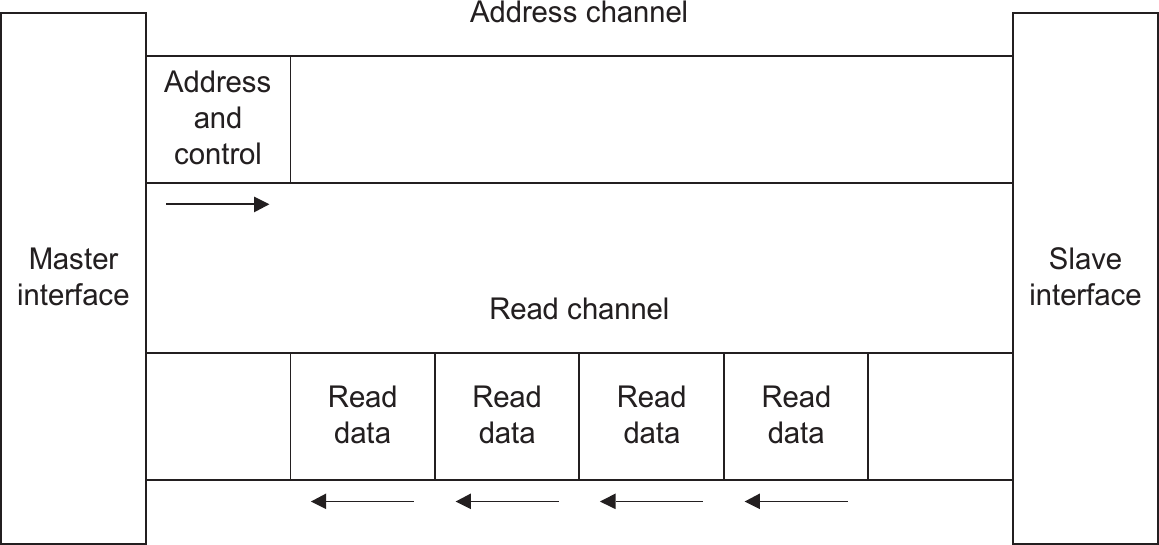
\includegraphics[width=0.9\textwidth,height=0.8\textheight,keepaspectratio]{axi_read}
		%\vspace*{-0.6cm}
		\source{Taken from \cite{axi_manual}}
	\end{figure}
	%\end{fullpage}
\end{frame}
%}}}

%{{{
\begin{frame}{AXI Write}
	%\begin{fullpage}
	\begin{figure}
		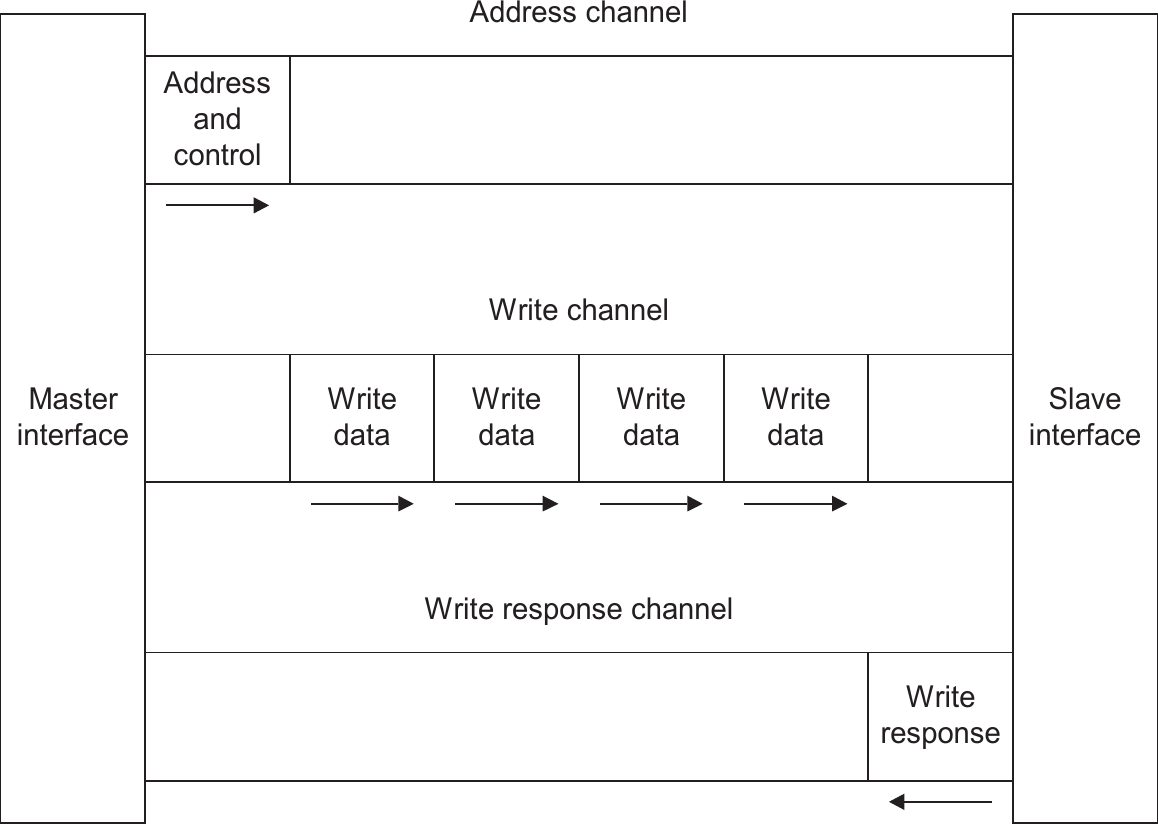
\includegraphics[width=0.9\textwidth,height=0.8\textheight,keepaspectratio]{axi_write}
		%\vspace*{-0.6cm}
		\source{Taken from \cite{axi_manual}}
	\end{figure}
	%\end{fullpage}
\end{frame}
%}}}

%{{{
\begin{frame}{AXI Features}
	%\begin{fullpage}
		\begin{columns}
			\column{0.47\textwidth}
			\begin{itemize}
				\item Handshake on all channels
				\item Burst up to 256 transfers
				\item Memory attributes
				\item Transaction buffering
			\end{itemize}
			\column{0.6\textwidth}
			\begin{itemize}
				\item Privileged, secure, instruction bits
				\item Transaction IDs
				\item Atomicy size
				\item Exclusive Access
				\item Quality of Service signals
			\end{itemize}
		\end{columns}
	%\end{fullpage}
\end{frame}
%}}}



%{{{
\begin{frame}{TileLink: Cache coherence network}
	\begin{itemize}
		\item Agents\\
			\begin{description}
				\item[Client] Request/hold \$ block
				\item[Manager] Oversee permission and data flow
			\end{description}
		\item Channels\\
			\begin{description}
				\item[Aquire] Start read/write uncached
				\item[Probe] Check if client has \$-block/revoke permissions
				\item[Release] Free data/write back
				\item[Grant] Provide data/permissions
				\item[Finish] Final acknowledgement from requestor
			\end{description}
			Refer to the specification for definitions of the exact operations
	\end{itemize}
\end{frame}
%}}}

%{{{
\begin{frame}{TileLink: Cache coherence network}
	\begin{fullpage}
	%{{{
		\only<1>{%
			\begin{figure}
				\showreqfalse
				\showwbfalse
				%\centering
				\inputimage{image3}%
			\end{figure}
		}
	%}}}
	%{{{
		\only<2>{%
			\begin{figure}
				\showreqtrue
				\showwbfalse
				%\centering
				\inputimage{image3}%
			\end{figure}
		}
	%}}}
	%{{{
		\only<3-4>{%
			\begin{figure}
				\showreqtrue
				\showwbtrue
				%\centering
				\inputimage{image3}%
			\end{figure}
		}
	%}}}
	\pause
	\pause
	\pause
	\begin{description}
		\item[Manager] Don't accept transactions for in-flight blocks
		\item[Client] Don't release block with outstanding voluntary write-back
	\end{description}
	\end{fullpage}
\end{frame}
%}}}



%{{{
\begin{frame}{RocketChip Interfaces}
	\begin{figure}
		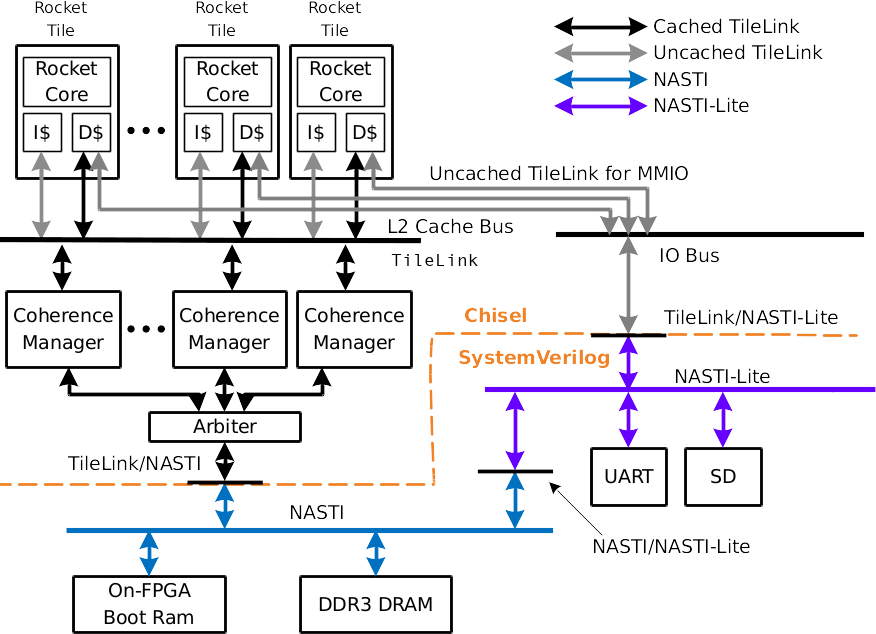
\includegraphics[width=\textwidth,height=0.8\textheight,keepaspectratio]{augmented_arch_edit}
		\vspace*{-0.6cm}
		\source{Clipped from \cite{lowrisc_techreport}}
	\end{figure}
\end{frame}
%}}}


%}}} End: section{Structure and Interfaces}


%{{{
\section[Conclusion]{Conclusion}


%{{{
\begin{frame}{Conclusion}
		\begin{columns}
			\column{0.5\textwidth}
			\begin{itemize}
				\item RISC-V is here to stay
				\item RocketChip generats SoC
				\item Can use Rocket or Boom
				\item Lots of configuration options
			\end{itemize}
			\column{0.5\textwidth}
			\begin{itemize}
				\item Chisel is hard to read
				\item Generated Verilog is worse
				\item RocketChip exposes AXI
				\item Many standard AXI IP
			\end{itemize}
		\end{columns}
\end{frame}
%}}}

%}}} End: section{}


%{{{ References

\center{References}
\tiny
\begin{thebibliography}{9}
	\bibitem{riscv_users}
		Some users of the RISC-V ISA\\
		lowRISC: \url{http://www.lowrisc.org/}; SiFive: \url{https://www.sifive.com/}\\
		Open-V: \url{https://www.crowdsupply.com/onchip/open-v} Pulp: \url{http://www.pulp-platform.org};\\
		IID Madras: \url{http://rise.cse.iitm.ac.in/shakti.html}\\
		Nvidia: \url{https://riscv.org/wp-content/uploads/2016/07/Tue1100_Nvidia_RISCV_Story_V2.pdf}\\
		UC Berkeley: \url{https://www.youtube.com/watch?v=WJndUQssFBg&t=1539s}\\

	\bibitem{rc_paper}
		Asanović, Krste/Avizienis, Rimas/Bachrach, Jonathan et at. (2016)\\
		The Rocket Chip Generator.\\
		Technical Report No. UCB/EECS-2016-17, EECS Department, University of California, Berkeley.\\
		\url{http://www2.eecs.berkeley.edu/Pubs/TechRpts/2016/EECS-2016-17.html}\\

	\bibitem{rc_github}
		The RocketChip github pages\\
		\url{https://github.com/ucb-bar/rocket-chip}\\
		\url{https://github.com/ucb-bar/project-template}\\

	\bibitem{boom_github}
		The Berkeley Out Of Order Machine github page\\
		\url{https://github.com/ucb-bar/riscv-boom}\\

	\bibitem{axi_manual}
		AXI Reference Guide, Xilinx 2011\\
		\url{http://www.xilinx.com/support/documentation/ip_documentation/ug761_axi_reference_guide.pdf}\\

	\bibitem{lowrisc_techreport}
		Xuan Guo, Nathanael Davison, Profir-Petru Partachi, Alistair Fisher (2016)\\
		Technical report from the lowRISC Summer Internship 2016\\
		\url{http://www.lowrisc.org/docs/internship-2016/report}\\

	\bibitem{axi_spec}
		AMBA® AXI™ and ACE™ Protocol Specification, ARM Limited 2011\\
		\url{http://infocenter.arm.com/help/topic/com.arm.doc.ihi0022d/index.html}\\
		\url{http://www.gstitt.ece.ufl.edu/courses/fall15/eel4720_5721/labs/refs/AXI4_specification.pdf}\\


	\bibitem{tile_link}
		The TileLink Specification, Version 0.3.3\\
		\url{https://docs.google.com/document/d/1Iczcjigc-LUi8QmDPwnAu1kH4Rrt6Kqi1_EUaCrfrk8/pub}

\end{thebibliography}
%}}}

%{{{ END

\begin{frame}{\Huge End}
	\huge Time for your questions
\end{frame}
%}}}

\end{document}
%}}}
